\documentclass[11pt,a4paper]{article}
\usepackage[utf8]{inputenc}
\usepackage[spanish]{babel}
\usepackage{amsmath}
\usepackage{amsfonts}
\usepackage{amssymb}
\usepackage{graphicx}
\usepackage[left=1.2cm,right=1.2cm,top=2cm,bottom=2cm]{geometry}
\date{\small{\today}}
\usepackage{fancyhdr}
\usepackage{afterpage}
\usepackage{titlesec}
\usepackage{float}
\usepackage{gensymb}
\usepackage{xfrac}
\usepackage{tabularx}
\usepackage{multicol}
\usepackage[font=small]{caption}
\usepackage{scrextend}
\usepackage[toc,page]{appendix}
\usepackage{tikz}
\usepackage{tkz-euclide}
\usepackage[siunitx,americanvoltages,fulldiodes]{circuitikz}
\usepackage{stackengine}
\usepackage{mathtools}
\usepackage{hyperref}
\DeclarePairedDelimiter\abs{\lvert}{\rvert}%
\DeclarePairedDelimiter\norm{\lVert}{\rVert}%
\usetikzlibrary{arrows}
\usepackage{caption}

\renewcommand\appendixpagename{Apéndices}
\renewcommand\appendixname{Apéndice}

\DeclareMathOperator{\arctantwo}{arctan2}

\titleformat{\section}{\Large\bfseries}{}{0em}{}[]
\titleformat{\subsection}{\large\bfseries}{}{0em}{}[]
\titleformat{\subsubsection}{\bfseries}{}{0em}{}[]
\titleformat{\chapter}{\large\bfseries}{}{0em}{}[]


\setlength\parindent{0pt}


\begin{document}
\title{Adaptación de Impedancia en Guía de Onda Rectangular}
	\LARGE{\textsc{Laboratorio II}}\\
	\Large{Adaptación de Impedancia en Guía de Onda Rectangular}\\
\begin{large}
\small\textsc{Bercic, Jerónimo}\\
\small\textsc{Roqueta, Matías Daniel}\\
\small{Instituto Balseiro, Centro Atómico Bariloche, Comisión Nacional de Energía Atómica}\\
\end{large}
\setcounter{page}{1}

\lhead{Laboratorio II}%Materia
\rhead{Adaptación de Impedancia en Guía de Onda Rectangular}%Título 
\chead{}

\lfoot{J. Bercic, M. Roqueta}
\cfoot{Instituto Balseiro} 
\rfoot{\thepage} 
\renewcommand{\headrulewidth}{0.4pt} 
\renewcommand{\footrulewidth}{0.4pt} 
\pagestyle{fancy}

\hrule
\normalsize
\section{Resumen}
Se midió la frecuencia de emisión de una fuente de microondas electromagnéticas $f=(10.53\pm0.05)$ GHz, y la longitud de onda de esta dentro de una guía de ondas rectangular WR90 de dimensiones $2,3\, \mathrm{cm} \times 1\, \mathrm{cm}$, obteniendo $\lambda_g=(3.97\pm0,02)$ cm. 
En estas condiciones se construyó un sistema de comunicaciones emisor-receptor, evaluando el efecto del receptor sobre la impedancia del emisor.
Sobre el sistema se realizó adaptación de impedancia, verificando que la señal transmitida hacia el receptor máxima si el emisor se encuentra en condición de impedancia adaptada. 

\begin{multicols}{2}
\section{Introducción}
Una guía de ondas electromagnéticas es un dispositivo que se utiliza para restringir los modos de emisión de una onda, y que esta sea propagada en una dirección deseada. De esta manera se puede aprovechar dicha energía de manera más eficiente. Su utilidad es evidente, por ejemplo, en la fabricación de antenas, donde se busca que la propagación sea en una dirección específica y que las pérdidas de información sean mínimas. \\

Las guías de onda pueden tener varias geometrías, una de las cuales es la guía de ondas rectangular caracterizada por su dimensión horizontal $a$ y su dimension vertical $b$. Esta guía puede propagar modos TE\textsubscript{mn} (Transverse Electric Field) y TM\textsubscript{mn} (Transverse Magnetic Field), que se refieren a si la onda transversal a la dirección de propagación es la eléctrica o la magnética. 
Respectivamente, \textbf{m} es el número de medias-ondas en dirección horizontal, y \textbf{n} es el número de medias-ondas en dimensión vertical. 
La figura \ref{fig:te10} presenta un esquema del modo TE$_{10}$ en una guía de ondas rectangular.
\begin{figure}[H]
    \centering
    \includegraphics[width=0.5\linewidth]{Images/TE10.jpg}
    \caption{Líneas de campo del modo TE$_{10}$ en una guía de ondas rectangular. En rojo las líneas de campo magnético y en azul las líneas de campo eléctrico.}
    \label{fig:te10}
\end{figure}
Estos modos de propagación dependerán tanto de las dimensiones de la guía, así como de la frecuencia de la onda propagada. 
A cada modo \textbf{mn} propagando en una guía rectangular corresponde una frecuencia de corte determinada por
\begin{equation}
    f_c = \frac{c}{2}\sqrt{\frac{m^2}{a^2}+\frac{n^2}{b^2}}
\end{equation}
Un modo \textbf{mn} propaga únicamente a frecuencias $f>f_c$.\\

Para caracterizar la guía de ondas se puede estudiar una gúia de ondas propagando determinado modo como una línea de transmisión, una cascada de cuadripolos (Figura \ref{fig:cuadri}) distribuidos a lo largo de la línea.
\begin{figure}[H]
\centering
\includegraphics[width=0.7\linewidth]{Images/linea de transm.jpeg}
\caption{Cuadripolo característico de una línea de transmisión arbitraria.}\label{fig:cuadri}
\end{figure}
La línea de transmisión cuenta con una impedancia característica $Z_0$, determinada por la ecuación \ref{eq:Zo}, donde la aproximación de línea de transmisión ideal equivale a considerar $R\rightarrow 0, \; G\rightarrow 0$.\cite{cheng_9}.

\begin{equation}\label{eq:Zo}
    Z_0=\sqrt{\frac{R+jwL}{G+jwC}}\xrightarrow{\quad\text{Línea Ideal} \quad}\sqrt{\frac{L}{C}}
\end{equation}\\[-1em]

Para una guía de onda operando en modo TE\textsubscript{mn} propagando una onda de frecuencia $f$, se cumple la relación
\begin{equation}
    Z_0=\frac{\lambda_g}{\lambda} Z_\text{vacío} = \frac{c}{f}\lambda_g Z_\text{vacío}
\end{equation}
Donde $Z_\text{vacío} = 376.6 \, \Omega$ es la impedancia característica del vacío, $\lambda_\text{vacío}$ 
es la longitud de la onda de frecuencia $f$ en el vacío, y $\lambda_g$ la longitud de la onda de frecuencia $f$ dentro de la guía.\cite{cheng_10}\\

Una línea de transmisión semi-infinita consiste en una línea de transmisión terminada en una impedancia de carga $Z_L$. 
La posición de $Z_L$ en la guía recibe el nombre de plano de carga, este genera una onda reflejada dentro de la guía según el coeficiente de reflexión $\Gamma$. 
\begin{equation}\label{eq:gamma}
    \Gamma = \frac{Z_\text{L}-Z_0}{Z_\text{L}+Z_0} 
\end{equation}
En particular $\Gamma = -1$ si $Z_L$ es un cortocircuito, $\Gamma = 1$ si $Z_L$ un circuito abierto, y $\Gamma = 0$ si $Z_L=Z_0$. La condición $Z_L=Z_0$ se llama impedancia adaptada y es la condición de máxima transferencia de potencia.\\ 

Generalmente se expresa la impedancia normalizada $z=\frac{Z}{Z_0}$. Con esta definición, la condición de impedancia adaptada se reduce a $z_L=1$.\\


Para verificar si $Z_L$ está adaptada, se analiza la onda estacionaria que se forma debido a la reflexión de la onda en el plano de carga (Figura \ref{fig:onda}). 
\begin{figure}[H]
    \centering
    \includegraphics[width=0.9\linewidth]{Images/onda vmax.jpg}
    \caption{Perfil de la onda estacionara en guía de ondas semi-infinita. El gráfico presenta voltaje en función de la posición. La recta vertical continua representa la posición del plano de carga, y la punteada la posición del mínimo más próximo a este.}
    \label{fig:onda}
\end{figure}
En particular, sus amplitudes máxima $V_\text{max}$ y mínima $V_\text{min}$. 
En función de ellas se define la ROE (razón de onda estacionaria) como
\begin{equation}\label{eq:roe}
    \text{ROE} = \frac{V_{max}}{V_{min}} = \frac{1+\abs{\Gamma}}{1-\abs{\Gamma}}
\end{equation}
Esta relación puede tomar valores dentro del rango $1<\text{ROE} < \infty$, y tiende a 1 en condición de impedancia adaptada. \\

La onda estacionaria es $\frac{\lambda_g}{2}$-periódica, y tendrá mínimos 
\begin{equation}
    x_k = \frac{\phi_\Gamma + 2 k\pi}{2\pi} \, \frac{\lambda_g}{2} \qquad  k\in\mathbb{Z}
\end{equation}

Se define el desplazamiendo del plano de carga $\delta$ como la ubicación del mínimo más próximo al plano de carga.\\

\subsection{Adaptación de Impedancia}

En una guía semi-infinta la impedancia en un plano varía en función de la distancia $x$ al plano de carga según la expresión,
\begin{equation}
    z(x) = \frac{1 + \Gamma e^{-j2kx}}{1 - \Gamma e^{-j2kx}}
\end{equation}
donde $k=\frac{2\pi}{\lambda_g}$ es el número de onda, y $j=\sqrt{-1}$.\cite{cheng_9} \\

Es equivalente trabajar con la admitancia normalizada en función de la distancia $y(x)$,
\begin{equation}
    y(x) = \frac{1}{z(x)} = \frac{1 - \Gamma e^{-j2kx}}{1 + \Gamma e^{-j2kx}}
\end{equation}
Esta expresión permite calcular la admitancia de entrada de dos guías en paralelo,
\begin{figure}[H]
    \centering
    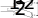
\includegraphics[width=0.6\linewidth]{Images/guiapll.pdf}
    \caption{Paralelo de dos guías de onda. La admitancia de entrada del paralelo cumple $y_\parallel = y_1+y_2$.}
    \label{fig:pll}
\end{figure}

El método de adaptación de impedancia con adaptador en paralelo consiste en:
\begin{enumerate}
    \item Encontrar en la guía un punto $x = \ell$ tal que la resistencia en $\ell$ esté normalizada, o sea que $y_1(\ell)=1+jb$.
    \item Colocar en $x=\ell$ una admitancia en paralelo puramente reactiva, de valor $y_a = -jb$.
\end{enumerate}

De esta forma se genera a la entrada del paralelo un nuevo plano de carga con admitancia adaptada 
$$y_L' = y(\ell) + y_a = 1$$

Los métodos para encontrar $\ell$ e $y_a$ pueden ser analíticos, numéricos\footnote{Un tal método es implementado y presentado el Apéndice 1.}, o usando la carta de Smith \footnote{Este método gráfico es presentado en el Apéndice 2.\cite{smith_1969}}.\\

En este trabajo de laboratorio, se busca medir las propiedades de la onda estacionaria que se forma bajo distintas condiciones del plano de carga. Además, se busca adaptar la impedancia a la vez que se mide la señal transmitida.
\section{Método Experimental}
Para este trabajo de laboratorio se utilizó una guía de ondas rectangular WR90, de dimensiones nominales $2,3\, \mathrm{cm} \times 1\, \mathrm{cm}$, resultando en frecuencias de corte
\begin{equation}
    f_{c_{10}} = 6,5\, \mathrm{GHz} \qquad f_{c_{20}}=13\,\mathrm{GHz}
\end{equation} 
Como fuente se utilizó un diodo Gunn, cuyo rango de emisión está entre 8 GHz y 12 GHz. 
Estos parámetros implican que la onda propagada por la guía sea una microonda, y que el modo de propagación corresponda al TE$_{10}$ (Figura \ref{fig:te10}).\\

Para medir se utilizan multímetros RIGOL DM3068. Las mediciones se registran en Python. \\


Primero se determina la frecuencia $f$ de emisión de la fuente, usando la línea de transmisión de la figura \ref{fig:arr1}.
\begin{multicols}{2}
    \begin{labeling}{III} 
        \item [I] Emisor Diodo Gunn
        \item [II] Aislador
        \item [III] Atenuador 3 dB
        \item [IV] Cavidad Resonante
        \item [V] Diodo detector
        \item [VI] Cortocircuito Móvil
    \end{labeling}        
\end{multicols}
\begin{figure}[H]
    \centering
    \includegraphics[width=0.9\linewidth]{Images/arreglo1.pdf}
    \caption{Línea de transmisión para medir frecuencia de emisión. La cavidad resonante actúa como filtro, absorbiendo su frecuencia de resonancia y dejando pasar otras frecuencias.}
    \label{fig:arr1}
\end{figure}
Se ajusta el cortocircuito móvil hasta detectar un máximo de onda estacionaria con el diodo detector, y se procede a ajustar la frecuencia de resonancia de la cavidad hasta que esta coincida con la frecuencia de emisión de la fuente.

\begin{figure}[H]
    \centering
    \includegraphics[width=0.9\linewidth]{Images/arreglo2.pdf}
    \caption{Linea de transmisión para medir longitud de onda. La terminación en cortocircuito provoca una onda estacionaria en la guía, la onda estacionaria se mide con una antena detectora en una línea ranurada.}
    \label{fig:arr2}
\end{figure}

Conociendo la frecuencia de operación del emisor, se procede a caracterizar la longitud de onda $\lambda_g$ dentro de la guía y su impedancia característica $Z_0$ usando la línea de transmisión de la figura \ref{fig:arr2}. La línea se termina en cortocircuito usando una placa de cobre.\\


Sobre la guía se dispone una antena móvil en la línea ranurada, que se desplaza con un carrito controlado por una placa de Arduino. 
La antena mide el voltaje eficaz en función de la posición, obteniendo el perfil de la onda estacionaria dentro de la guía.\\ 

Una vez conocidas $\lambda_g$ y $Z_0$, se puede proceder a adaptar impedancias. Se costruye la línea de transmisión correspondiente a la Figura \ref{fig:arr4}.

\begin{figure}[H]
    \centering
    \includegraphics[width=\linewidth]{Images/arreglo4.pdf}
    \caption{Sistema de adaptación de impedancias para una impedancia de carga $Z_L$, un tornillo capacitivo actúa como adaptador en paralelo.}
    \label{fig:arr4}
\end{figure}

Se sigue el siguiente procedimiento para la adapatación de impedancia

\begin{enumerate}
    \item Se mide la onda estacionaria con $Z_L$ en cortocircuito, referenciando el plano de carga a un mínimo de onda estacionaria.
    \item Se cambia $Z_L$ por una impedancia arbitraria y se mide la onda estacionaria. Se calculan la ROE y el desplazamiento $\delta$ del plano de carga.
    \item Usando la ROE y el desplazamiento del plano de carga, se calcula la posición del adaptado $\ell$ y su admitancia $y_a$. 
    Estos cálculos se realizan tanto con la carta de Smith como numéricamente.
    \item Se ajusta la posición y admitancia\footnote{La admitancia se determina por la profundidad del mismo dentro de la guía, según la tabla del apendice 2\\[-2em]} del adaptador, se mide nuevalente la ROE validando su disminución ante impedancia adaptada.
\end{enumerate}

Este método de adaptación de impedancia se utiliza para adaptar la impedancia en el sistema transmisor-receptor representado en la Figura \ref{fig:sistema}

\begin{figure}[H]
    \centering
    \includegraphics[width=\linewidth]{Images/sistema.pdf}
    \caption{Sistema transmisor-receptor.
    \texttt{Tx:} línea de la figura \ref{fig:arr4} con antena de bocina en $Z_L$. 
    \texttt{Rx:} detector de señal adaptado con una antena de bocina.}
    \label{fig:sistema}
\end{figure}

El sistema se adapta con el siguiente procedimiento
\begin{enumerate}
    \item Se retira el módulo Rx y se mide la ROE, validando que la antena de bocina adapta la impedancia de la guía a la impedancia del espacio libre.
    \item Se ubica el módulo Rx a 10 cm del módulo Tx. Se mide la ROE, observando el incremento de la misma respecto a la medición anterior.
    \item Se realiza el procedimiento de adaptación de impedancia en presencia del módulo Rx.
\end{enumerate}

Se registra la intensidad de señal medida por Rx antes y después de adaptar impedancia.

\section{Resultados}
Para la frecuencia de trabajo de la fuente, se obtuvo un valor de 
$$
f = (10.53 \pm 0.05) \text{ GHz}
$$
La medición es consistente con el valor provisto por el fabricante de $f_\text{f}=10.5$ GHz. \\

Se procede a medir la longitud de onda con la línea en cortocircuito, presentando el perfil de la onda estacionaria resultante en la Figura \ref{fig:cortocir}
\begin{figure}[H]
    \centering
    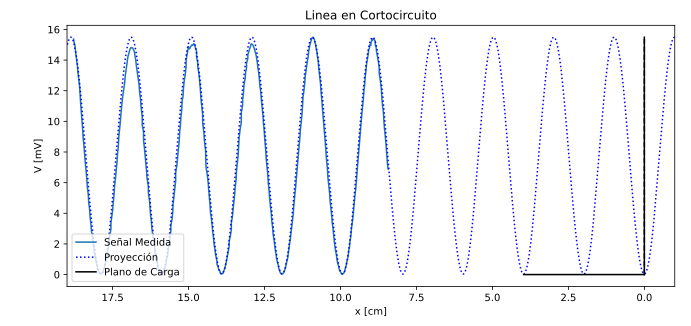
\includegraphics[width=\linewidth]{Images/lineacc.pdf}
    \caption{Perfil de la onda estacionaria cuando $Z_L$ es una placa de cobre. En azul continuo se presentan los datos medidos, en azul punteada su función de ajuste. La recta negra vertical representa la referencia del plano de carga y la recta roja horizontal el valor medido de $\lambda_g$.}
    \label{fig:cortocir}
\end{figure}

La longitud de onda dentro de la guía resulta
$$
\lambda_\text{g} = (3.97 \pm 0,02) \text{ cm} 
$$
La impedancia característica de la guía se calcula con la ecuación \ref{eq:Zo}
\begin{equation}\label{eq:Zo_medido}
    Z_0 = (526 \pm 3) \text{ } \Omega   
\end{equation}

\subsection{Adaptación de Impedancia}

Luego de reemplazar la placa por la antena de bocina en el plano de carga como se muestra en la Figura \ref{fig:sistema}, se obtuvo el siguiente perfil de onda (Figura \ref{fig:bocina}),
\begin{figure}[H]
    \centering
    \includegraphics[width=\linewidth]{Images/antena_bocina.pdf}
    \caption{Perfil de la onda estacionaria cuando $Z_L$ es una antena de bocina frente al espacio libre.}
    \label{fig:bocina}
\end{figure}
Se miden la ROE y el desfasaje del plano de carga
$$
\text{ROE} = 1.19 \pm 0.02  \qquad \delta = (0.009 \pm 0.003)\lambda_g
$$
Correspondientes a una impedancia de carga de
$$
Z_L = \left[(472 \pm 0.840) - j (9 \pm 3)\right] \,\Omega
$$
Notar que es similar al valor de $Z_0$ presentado en el resultado \ref{eq:Zo_medido}, indicando impedancia adaptada. Luego de colocar el módulo receptor según la figura \ref{fig:arr4}, se mide nuevamente la onda estacionaria, obteniendo
$$
\text{ROE} = 14.0\pm0.4 \qquad \delta = (0.063 \pm 0.007)\lambda_g
$$
Correspondientes a una impedancia de carga de
$$
Z_L = \left[(47\pm2) - j (232 \pm 3)\right]\,\Omega
$$
Verificando que la presencia del módulo receptor frente al emisor desadaptó la impedancia\\

Con estos datos, se calcula la admitancia necesaria del adaptador y su posición sobre la guía con el método numérico y con la carta de Smith
$$
y_a \simeq 3.4j \qquad\qquad \ell \simeq 7.8 \text{ cm}
$$

Ubicando el adaptador de impedancia se mide nuevamente la onda estacionaria, obteniendo
$$
\text{ROE} = 1,15 \pm 0,01 \qquad \delta = (0.072 \pm 0.005)\lambda_g
$$
Correspondientes a una impedancia de carga de
$$
Z_L = \left[(512\pm5) - j (57 \pm 4)\right]\,\Omega
$$
Nuevamente se aproxima a el valor de $Z_0$ medido, verificando que se recuperó la condición de impedancia adaptada.\\

Se muestra en la Figura \ref{fig:bocirec} la comparación de onda estacionara medida ante impedancia adaptada y desadaptada, validando la disminución en amplitud de la onda estacionaria por adaptación de impedancia. 
\begin{figure}[H]
    \centering
    \includegraphics[width=\linewidth]{Images/bocina_receptor.pdf}
    \caption{En azul, el perfil de onda estacionaria con impedancia desadaptada. 
    En naranja, el perfil de la onda estacionaria con la impedancia adaptada. 
    La línea vertical continua es la referencia plano de carga, y la vertical punteada el desfasaje del plano de carga.}
    \label{fig:bocirec}
\end{figure}

Y, en la Figura \ref{fig:senal}, se grafica el voltaje medido por la antena con la guía desadaptada, en contraste con el voltaje medido por la guía adaptada,
\begin{figure}[H]
    \centering
    \includegraphics[width=\linewidth]{Images/señal_transmitida.pdf}
    \caption{En azul, la señal medida por el Rx en función del tiempo, con la guía desadaptada. En naranja, la misma con la guía adaptada.}
    \label{fig:senal}
\end{figure}

Con la impedancia adaptada se mide en la antena receptora una tensión eficaz de $v_a = (2.01 \pm 0.01)$ mV, mientras que con la impedancia desadaptada se miden $v_d = (1.47\pm0.02)$ mV. Se calcula la pérdida en intensidad de señal por la impedancia desadaptada
\begin{equation*}
    \frac{v_{d}}{v_{a}} = 0.74 \pm 0.1
\end{equation*}

\section{Discusión}


El experimento verificó que la antena de bocina actúa como un buen adaptador de impedancias de la guía de ondas al espacio libre, que se ve reflejado en una medición de la ROE crecana a 1. \\

Sin embargo, este es sensible a la presencia de objetos próximos a la antena, ya que estos generan una onda reflejada, lo que se manifiesta en un incremento significativo de la ROE en presencia del módulo receptor.\\

La presencia del receptor se puede modelizar como una modificación de la impedancia de carga sobre la guía, que se puede corregir con adaptación de impedancias.\\

Se puede notar que, luego de la adaptación de la guía en presencia del receptor, la ROE recupera un valor cercano a 1, indicando que la adaptación fue exitosa. \\

El incremento en el voltaje medido por el receptor se ve incrementado luego de la adaptación implica que mayor señal está siendo transmitida, como era de esperar.\\

\section{Conclusiones}

Los métodos de adaptación de impedancia usados, método numérico y por carta de Smith, retornaron resultados consistentes, verificando que son equivalentes.\\

La adaptación de impedancias con los valores de $\ell$, $y_a$ retornados por estos métodos generaron una disminución significativa de la ROE en un sistema desadaptado, verificando experimentalmente su validez.\\


Luego de la adaptación de impedancia, se midió un incremento en la señal transmitida al receptor por la guía. Debido a esto, se concluye que la adaptación de impedancias conduce a una mayor transferencia de potencia. \\


\bibliography{Waveguide}
\bibliographystyle{unsrt}

\end{multicols}
\newpage
\begin{appendices}
\vspace{-1em}
\hrule
\vspace{1em}
\normalsize
\section{Apéndice 1 - Resolución Numérica con Python}
\begin{multicols}{2}
    Se registra un vector de mediciones experimentales de la onda estacionaria \texttt{[x, v]}, de estos datos se extraen

    \begin{equation}
        \mathtt{vmax} = \mathtt{max(v)} \qquad \qquad \mathtt{vmin} = \mathtt{min(v)}
    \end{equation}\\[-1em]

    Los datos se ajustan a la función \ref{eq:fit} que aproxima el perfil de la onda estacionaria, de carácter $\frac{\lambda_g}{2}$-periódico.

    \begin{equation}\label{eq:fit}
        \mathtt v = A_0 -A\cos(2k\mathtt x-\phi)
    \end{equation}\\[-1em]

    Donde $A$ y $A_0$ se calculan a partir de \texttt{vmax} y \texttt{vmin}, y $k = \frac{2\pi}{\lambda_g}$, dejando a $\phi$ como parámetro de ajuste.\\

    A partir de estos datos se calculan la razón de onda estacionaria y el desplazamiento del plano de carga

    \begin{equation}
        \mathrm{ROE} = \frac{\mathtt{vmax}}{\mathtt{vmin}}\qquad\qquad\delta = \frac{\phi}{2\pi}\,\frac{\lambda_g}{2}
    \end{equation}\\[-1em]

    Notar que el valor de $\mathtt{x} = \delta$ es el que minimiza la función de ajuste \ref{eq:fit}. A continuación el procedimiento es equivalente al procedimiento gráfico realizado con la carta de Smith, presentado en el Apéndice 2.\\

    A partir de la ROE y $\delta$, se calcula el coeficiente de reflexión $\Gamma = \left|\Gamma\right|e^{j\phi_\Gamma}$ a partir de su módulo y fase

    \begin{equation}
        \left|\Gamma\right| = \frac{\mathrm{ROE}-1}{\mathrm{ROE}+1}\qquad\qquad \phi_\Gamma = \pi-2k\delta
    \end{equation}\\[-1em]

    \begin{figure}[H]
        \centering
        \includegraphics[width=\linewidth]{Images/ydex.pdf}
        \caption{Gráfico superior: Conductancia normalizada y recta $g=1$, intersecciones con la recta $g=1$ son candidatos a adaptacion de impedancia.
            Gráfico inferior: Suceptancia normalizada y recta $b=0$, suceptancias negativas son inductivas y suceptancias positivas son capacitivas.}
        \label{fig:ydex}
    \end{figure}
    Teniendo el valor de $\Gamma$ se expresa la admitancia normalizada en función de la distancia al plano de carga a partir de la ecuación \ref{eq:y_normal}. La admitancia se grafica en su parte real e imaginaria y se presenta en la figura \ref{fig:ydex}\\

    Se define un margen de tolerancia $\epsilon = 0.01$\footnote{Se define un márgen de tolerancia debido al error de discretización}, y se itera sobre los índices \texttt{i} de \texttt{y}, seleccionando aquellos que cumplen las siguientes condiciones

    \begin{itemize}
        \item La conductancia normalizada es igual a 1 dentro del margen de tolerancia
        $$\mathtt{ 1-\epsilon \le np.real(y[i]) \le  1+\epsilon}$$
        \item Debido a que el adaptador en paralelo es capacitivo, la suceptancia en la guía necesita ser inductiva
        $$\mathtt{np.imag(y[i])< 0}$$
    \end{itemize}

    A partir de los índices \texttt{i} que cumplen estas dos condiciones simultaneamente se obtienen la posición $\ell$ del adaptador capacitivo y la admitancia de este $y_a$ 
    
    \begin{equation}
        \mathtt{\ell = x[i]\qquad\qquad y_a = - np.imag(y[i])}
    \end{equation}\\[-1em]

    Se informan el valor de $y_a$ y los posibles valores que puede tomar $\ell$, estos además se grafican junto a la admitancia normalizada en la figura \ref{fig:ydex_l}\\

    \begin{figure}[H]
        \centering
        \includegraphics[width=\linewidth]{Images/ydex_l.pdf}
        \caption{Gráfico \ref{fig:ydex} argegando en línea punteada vertical las posibles ubicaciones en la guía que puede tomar un adaptador de impedancias capacitivo.}
        \label{fig:ydex_l}
    \end{figure}

\end{multicols}
\pagebreak
\section{Apéndice 2 - Resolución con Carta de Smith.}
\begin{multicols}{2}
    Se encuentran los valores de la relación de onda estacionaria y el desplazamiento del plano de carga con el mismo método ilustrado en el Apéndice 1.\\
    
    Estos valores se usan para trazar el círculo $\left|\Gamma\right|$ y la recta $\phi_\Gamma$ en la carta de Smith, obteniendo la figura \ref{fig:smith1}
    \begin{figure}[H]
        \centering
        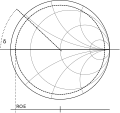
\includegraphics[width=0.8\linewidth]{Images/smith1.pdf}
        \caption{Trazas iniciales a partir de las mediciones de ROE y $\delta$ en la carta de Smith, correspondientes a determinado $\Gamma$.}
        \label{fig:smith1}
    \end{figure}
    La intersección entre el círculo $\left|\Gamma\right|$ y la recta $\phi_\Gamma$ permiten encontrar las coordenadas de $z_L$. Extendiendo la recta $\phi_\Gamma$ hasta el extremo opuesto del diagrama encuentra las coordenadas de $y_L$ obteniendo la figura \ref{fig:smith2}
    \begin{figure}[H]
        \centering
        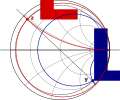
\includegraphics[width=0.8\linewidth]{Images/smith3.pdf}
        \caption{Coordenadas de $z_L$ en rojo e $y_L$ en azul en la carta de Smith, correspondientes a determinado $\Gamma$.}
        \label{fig:smith2}
    \end{figure}

    Teniendo las coordenadas de $y_L$ se puede encontrar el $x$ que satisface $y(x)=1+jb$. Esto se consigue recorriendo el círculo de radio $\left|\Gamma\right|$ hasta su intersección con el círculo $g=1$.
    Al existir dos tales intersecciones, se elige la inductiva, que en la carta de Smith significa estar en la mitad inferior del diagrama. Reflejada a esta verticalmente está la admitancia que necesita el adaptador en paralelo $y_a$, presentadas en la figura \ref{fig:smith3}.

    \begin{figure}[H]
        \centering
        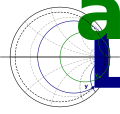
\includegraphics[width=0.8\linewidth]{Images/smith2.pdf}
        \caption{Método para encontrar $y_a$ con la carta de Smith. En verde las coordenadas de $y$ necesitadas en el punto $\ell$ y en verde punteada la admitancia en paralelo que las compensa. Recorrer el círculo de radio $|\Gamma|$ equivale a recorrer los valores de $y$ en la figura \ref{fig:ydex} del Apéndice 1.}
        \label{fig:smith3}
    \end{figure}
    Finalmente se mide la distancia al plano de carga $\ell$ en unidades de $\lambda_g$ midiendo la distancia angular desde la recta que pasa por $y_L$ hasta la que por $y$ en sentido antihorario como indica la figura \ref{fig:smith4}.
    \begin{figure}[H]
        \centering
        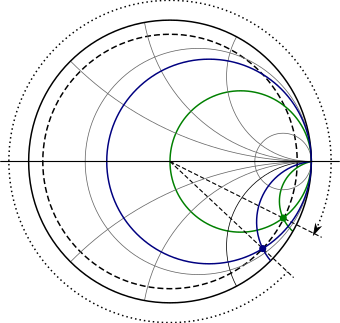
\includegraphics[width=0.8\linewidth]{Images/smith4.pdf}
        \caption{Valor de $\ell$ en unidades de $\lambda_g$ representado como distancia angular en la Carta de Smith. Equivale a la primer recta vertical en la figura \ref{fig:ydex_l} del Apéndice 1.}
        \label{fig:smith4}
    \end{figure}


\end{multicols}

\pagebreak
\section{Apéndice 3 - Determinación de la profundidad de inserción del tornillo adaptador en la guía de ondas.}
Para determinar con qué profundidad se debe insertar el tornillo adaptador en la guía, se utiliza el diagrama de la 
Figura \ref{fig:torni} 
\begin{figure}[H]
    \centering
    \includegraphics[scale=0.75]{Images/Apendice 2.jpg}
    \caption{Cociente entre la profundidad $s$ y el alto de la guía $b$, en función de la susceptancia normalizada $Y_1$}
\end{figure}\label{fig:torni}
Este diagrama se extrajo del libro \textit{Introductory Waveguide Techiques}, de Richard W. Tinnell.\cite{tinnell_1974}

\end{appendices}


\begin{multicols}{2}

\end{multicols}

\end{document}